\begin{figure*}[t]
    \begin{minipage}{0.8\textwidth}
        \centering
        \begin{subfigure}[b]{0.3\linewidth}
            \includegraphics[width=\textwidth]{ICLR_2025/Figures/appx_rigid_pushing/rigid-pushing-task.png}
        \end{subfigure}
        \hspace{0.2cm}
        \begin{subfigure}[b]{0.45\linewidth}
            \includegraphics[width=\textwidth]{ICLR_2025/Figures/appx_rigid_pushing/eval_30_Isaac-Rigid-Pushing-No-Contact-Multi-v0_eval_all.pdf}
        \end{subfigure}
    \end{minipage}
    \begin{minipage}{0.1\textwidth}
        \centering
        \hspace{-1.5cm}
        \makebox[\textwidth][c]{
        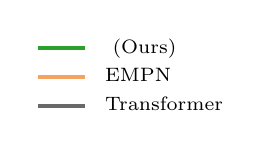
\begin{tikzpicture}
    \tikzstyle{every node}=[font=\scriptsize]
    \definecolor{tabblue}{RGB}{31, 119, 180}
\definecolor{taborange}{RGB}{255, 127, 14}
\definecolor{tabgreen}{RGB}{44, 160, 44}
\definecolor{tabred}{RGB}{214, 39, 40}
\definecolor{tabpurple}{RGB}{148, 103, 189}
\definecolor{tabbrown}{RGB}{140, 86, 75}
\definecolor{tabpink}{RGB}{227, 119, 194}
\definecolor{tabgray}{RGB}{127, 127, 127}
\definecolor{tabolive}{RGB}{188, 189, 34}
\definecolor{tabcyan}{RGB}{23, 190, 207}
\definecolor{lightblue}{RGB}{173, 216, 230}
\definecolor{sandybrown}{RGB}{244, 164, 96}
\definecolor{darkgrey}{RGB}{169, 169, 169}
\definecolor{dimgrey}{RGB}{105, 105, 105}
\definecolor{olivedrab}{RGB}{107, 142, 35}
\definecolor{darkviolet}{RGB}{148, 0, 211}
\definecolor{darkgoldenrod}{RGB}{184, 134, 11}
\definecolor{darkblue}{RGB}{0, 0, 139}
\definecolor{orchid}{RGB}{218, 112, 214}

    \begin{axis}[%
        hide axis,
        xmin=10,
        xmax=50,
        ymin=0,
        ymax=0.1,
        legend style={
            draw=white!15!black,
            legend cell align=left,
            legend columns=1,
            legend style={
                draw=none,
                column sep=1ex,
                line width=1pt,
            }
        },
        ]
        \addlegendimage{line legend, tabgreen, ultra thick} % Thicker line here
        \addlegendentry{\textbf{\model} (Ours)}
        \addlegendimage{line legend, sandybrown, ultra thick} % Thicker line here
        \addlegendentry{EMPN}
        \addlegendimage{line legend, dimgrey, ultra thick} % Thicker line here
        \addlegendentry{Transformer}
    \end{axis}
\end{tikzpicture}
        }
    \end{minipage}
    
    \caption{\rebuttal{\textbf{Left:} Rigid-Pushing task, where a rod is controlled in the $x$-$y$ plane to push an object to a desired target position and orientation. \textbf{Right:} Performance comparison between HEPi and baseline models over 10 seeds. HEPi outperforms both baselines by effectively exploiting task symmetries and modeling heterogeneity.}
    }
    \vspace{-0.2cm}
    \label{fig:rigid_pushing_task}
\end{figure*}
